\lab{Algorithms}{Interior Point I}{Interior Point I}
\objective{Learn About Interior Point Methods for Linear Programming}

\section*{Interior Point Methods: Overview}
Although the Simplex Algorithm was long the only practically competitive method for linear programming, the past 30 years has seen the discovery and widespread adoption of a new family of algorithms that rival and in some cases outperform the Simplex Algorithm, collectively called Interior Point methods. One of the major shortcomings of the Simplex Algorithm is that the number of steps required to solve the problem can grow exponentially in the size of the linear system. Thus, for certain large linear programs, the Simplex Algorithm is simply not viable. In practice, however, such pathological examples are rarely encountered. Interior Point methods offer and alternative approach and guarantee much better theoretical convergence properties.

Recall that a linear program is a constrained optimization problem with a linear objective function and linear constraints.
The linear constraints define a set of allowable points called the \emph{feasible region}, the boundary of which forms a geometric
object known as a \emph{polytope}. The theory of convex optimization ensures that the optimal point for the objective function
can be found among the vertices of the feasible polytope. The Simplex Method tests a sequence of such vertices until it finds 
the optimal point. Provided the linear program is neither unbounded nor infeasible, the algorithm is certain to produce the correct
answer after a finite number of steps, but it does not guarantee an efficient path along the polytope toward the minimizer. Interior point methods do away with the feasible polytope and instead generate a sequence of points that cut through the interior (or 
exterior) of the feasible region and converge iteratively to the optimal point. Although it is computationally more expensive to 
compute such interior points, each step results in significant progress toward the minimizer. See Figure \ref{intPoint:intPath} for
a visualization of an Interior Point method. In general, the Simplex Method requires many more, albeit less expensive, computations.

\begin{figure}
\centering
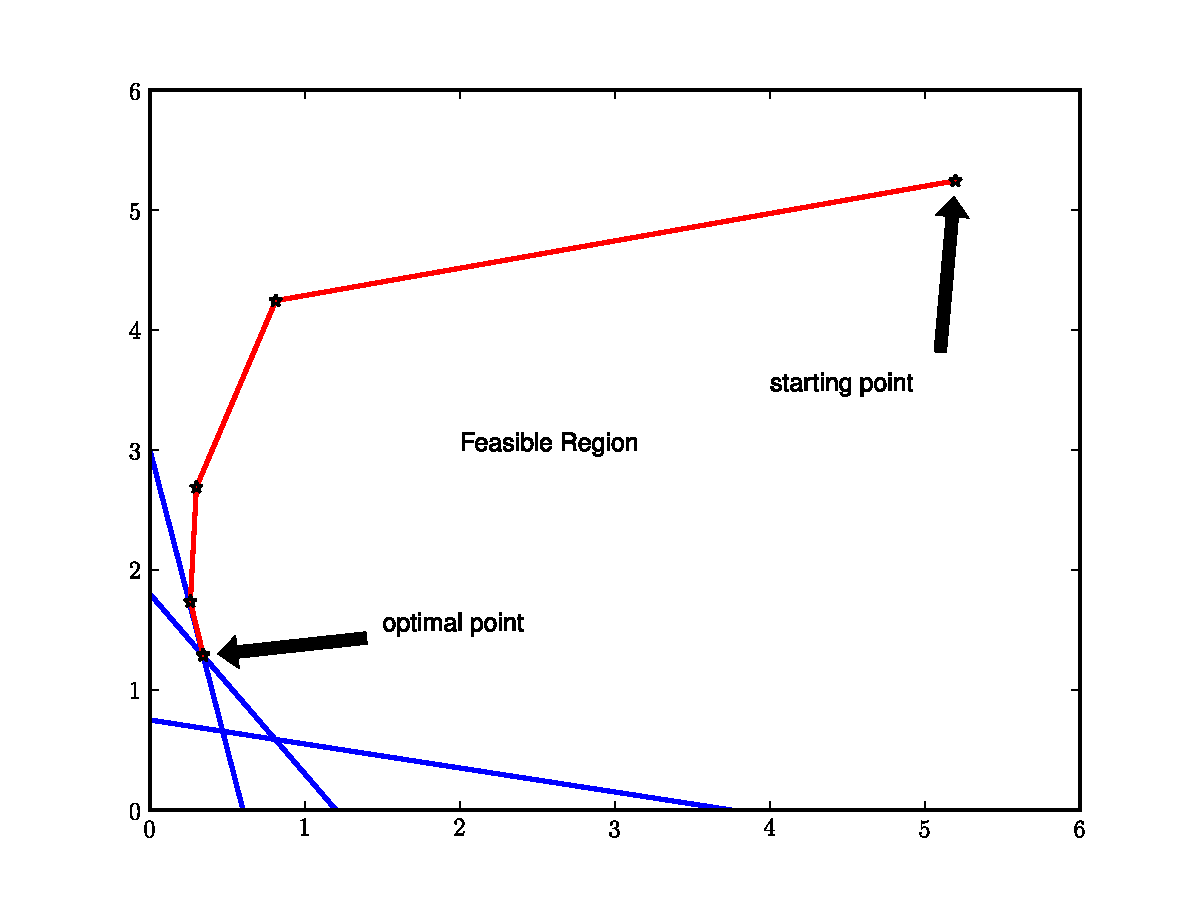
\includegraphics[width=\textwidth]{interiorPath.pdf}
\caption{A path traced by an Interior Point algorithm.}
\label{intPoint:intPath}
\end{figure}

\section*{Primal-Dual Interior Point Methods}
The most popular and successful types of Interior Point methods nowadays are known as Primal-Dual Interior Point methods. To 
describe this approach, let us consider the following linear program:
\begin{align*}
\text{minimize } &c^Tx\\
\text{subject to } &Ax = b\\
&x \geq 0.
\end{align*}
Here, $x, c \in \mathbb{R}^n$, $b \in \mathbb{R}^m$, and $A$ is an $m \times n$ matrix with full row rank. By $x \geq 0$, we 
simply mean that each coordinate of $x$ is nonnegative. Note that this formulation is quite general, as any linear program can be
posed in this manner, after appropriate transformations. This is the primal problem, and its dual takes the form
\begin{align*}
\text{maximize } &b^T\lambda\\
\text{subject to } &A^T\lambda + s = c\\
&s \geq 0,
\end{align*}
where $\lambda \in \mathbb{R}^m$ and $s \in \mathbb{R}^n$. The theory of convex optimization tells gives us necessary and sufficient
conditions for the solutions to the primal and dual problems via the Karush-Kuhn-Tucker conditions, which in this case take the form
\begin{align*}
A^T\lambda + s &= c\\
Ax &= b\\
x_is_i = 0, \,\,\, i = 1,2,\ldots,n\\
x, s \geq 0.
\end{align*}
Thus, if we can find a solution $(x^*, \lambda^*, s^*)$ to these equations, we have solved our original linear program. 
The top three lines of the KKT conditions can be re-written as one large almost-linear system equal to 0. In the spirit of
Newton's Method, we can form a linear approximation of this system centered around our current point $(x, \lambda, s)$, and
calculate the direction $(\triangle x, \triangle \lambda, \triangle s)$ in which to step in order to set the linear approximation 
equal to 0. This equates to solving the linear system
$$
\begin{bmatrix}
0 & A^T & I\\
A & 0 & 0\\
S & 0 & X
\end{bmatrix}
\begin{bmatrix}
\triangle x\\
\triangle \lambda\\
\triangle s
\end{bmatrix}
=
\begin{bmatrix}
-r_c\\
-r_b\\
-XSe
\end{bmatrix},
$$
where $r_b = Ax - b,$ $r_c = A^T\lambda + s - c$, $I$ is an appropriately-sized identity matrix, $X = \text{diag}(x_1,\ldots,x_n),$
$S = \text{diag}(s_1,\ldots,s_n)$, and $e = (1,1,\ldots,1)^T$. 
This Newton direction is too greedy, however, and even small steps in this direction may cause us to violate the nonnegativity
condition (the last line of the KKT conditions). To fix this, we introduce a 


Discuss the idea of barrier terms, changing a constrained problem into an unconstrained problem. It does complicate things, however, only allowing us to approximate the true optimal point. Adjusting the parameters of the barrier function (i.e. the scalar constant multiplied to the log terms) can improve accuracy. 